\chapter{相关工作}
% 本文研究课题为日常健康场景下的面诊系统设计与实现,面诊算法的具体实现细节不属于相关工作,本文主要关注面诊系统设计与日常交互设计。
为了更好地从交互设计以及系统设计层面,设计出适用于日常健康场景下的面诊系统,
本章将介绍当前比较流行的基于面诊技术的面诊系统以及当前人机交互领域中日常健康场景的相关研究。

\section{面诊系统}

% 目前已经有不少研究与面诊系统相关,

总的来说,面诊系统的发展随着技术的发展主要经历了三个阶段:
\begin{enumerate}
    \item 早期在读脸技术相对成熟的基础上,以面诊仪为代表面诊系统主要目的是提高传统面诊效率,为医护人员提供自动化的患者面部信息采集、面部特征提取的能力。
    \item 随着诊断理论客观化研究的进一步深入,诊断模型特别是基于深度学习的模型能力大大增强,面诊系统不再局限于只提供基本的特诊信息,开始关注自动分析诊断能力,辅助医护人员进行临床诊断。
    \item 近年来日常健康管理的逐渐兴起,人们对健康更加重视,越来越多研究开始关注如何辅助用户进行日常健康管理以满足用户的诉求。移动设备存储处理能力的提高也为各类系统日常化、便携化提供了基础。
    国内外出现为日常场景设计的健康管理系统,面诊系统也有从诊所环境迁移到日常场景的趋势,但相关研究还处于比较初级的阶段。
\end{enumerate}

这些研究的出发点不完全相同,经过梳理后本文将主要介绍代表性的几类,同时简单概括其特点以及不足之处。

% 介绍发展背景,面诊算法发展,阐述当前的技术发展
以往的面诊需要专业的医生观察患者的面部,结合各方面患者的综合情况,根据中医面诊理论得出最终的诊断结果。
传统面诊模式制约了中医的现代化推进,一方面,传统的面诊方式存在以下明显的缺点:(1) 效率低,需要专业医生参与。(2) 对医生的要求比较高,且易受到医生对患者身体状况主观判断的影响,结果可能不够客观;另一方面,随着中医信息化的推进,各诊所对标准化用户信息采集,电子病历等要求也越来越迫切,因此推动了传统面诊方式进行改革。
而在计算机领域,与面部信息相关的读脸技术也在快速发展,这为面诊系统提供了技术基础。读脸技术(Face Reading Technology)通过读取人的面部图片获取相关的信息,主要应用有人脸检测、人脸识别、情绪识别、性别识别、年龄识别等\cite{Schroff2015FaceNet, Zhang2016Joint, corneanu2016survey}。
基于面部图像分析的读脸技术在各领域的应用也越来越广泛如安全访问控制\cite{liu2005ibotguard}、身份识别\cite{he2015delving}、考勤管理\cite{surekha2017attendance}等。
其中,读脸技术医疗环境中应用也成为研究热点,如基于读脸技术获取定位面部区域、获取面色舌苔唇色等,这类技术在标准环境配合在对应硬件采集设备如光电血流容积仪,色差仪等,已经可以达到足够的精度。
面诊仪是基于以上读脸技术研发的一类面诊系统,面诊仪其主要目的是为了减轻医生的负担,同时在一定程度上将诊断依据客观化,避免人为的主观判断导致结果出现偏差\cite{李丹溪2017舌诊仪的发展及其在舌诊客观化研究中的应用现状}。
如图 \ref{fig:med}所示,道生面诊仪\cite{邸丹2016手持式舌象仪的研制}是目前某些医院用来采集面部信息的设备,芜湖圣美孚科技有限公司\footnote{http://www.smfkj.com/}也有一款舌面诊一体化设备。
这类系统利用色差仪、可以实现面部图像采集以及面部特征提取,如面色、唇色、舌苔、舌象等,为诊断提供依据。

\begin{figure}[h]
    \centering
    \subfigure[面诊仪]{
        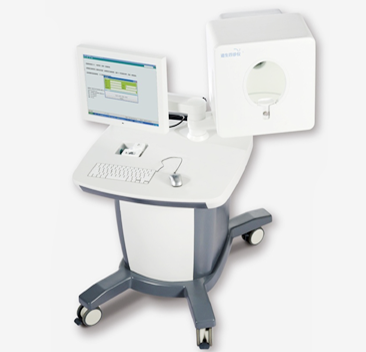
\includegraphics[width=5cm]{images/mzy.png}
    }
    \subfigure[舌面诊一体化设备]{
        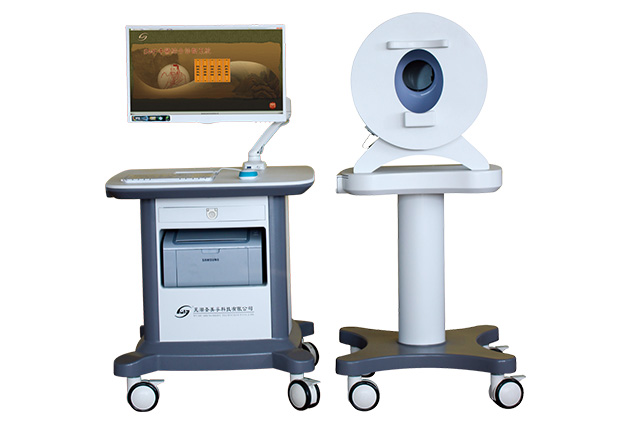
\includegraphics[width=5cm]{images/SMF.jpg}
    }
    \caption{面诊仪\cite{邸丹2016手持式舌象仪的研制}}
    \label{fig:med}
\end{figure}
% 介绍 面诊技术信息化 

早期的面诊仪可作为初步信息采集工具得到患者的面色,舌象等信息,但随着诊断理论客观化研究的发展,也有相关工作在面诊仪的基础上提供了一定的自动化分析诊断能力。
诊断理论客观化研究即使用计算机信息化技术,通过理论研究与实验研究,将传统与临床的诊断理论,系统地研究出其量化的本质,包括量化面色、舌象、脉搏信息与健康指标的关系\cite{Wang2013TCM, guo2015analysis, li2020tcminet},从而为其信息化应用提供基础。
在临床上,也有大量利用信息化技术进行关于面部信息与冠心病、慢性肾衰竭、脑血管病等相关分析,从而为诊断提供相应的辅助功能,如面色自动识别分析系统\cite{崔骥2018人工智能背景下中医诊疗技术的应用与展望}则能得出初步的诊断结果,然后由医生再根据这些信息得到最终结果,在一定程度上减少了医生工作的负担。
除面诊仪外,在中医面诊标准化、客观化、信息化的基础上,不少基于中医面诊理论的面诊系统也随之出现。
常见的基于中医的面诊管理系统,其设计的初衷是在诊所的标准环境下服务于医护人员。上海中医药大学的李福凤等基于中医望诊装置\cite{李国正0一种用于中医望诊的三维图像采集装置}的基础上,
利用模式识别相关算法,通过面部分割,面色、光泽、口唇特征分析等方法,实现了一个中医面诊分析与诊断系统\cite{李福凤2016中医面诊分析与诊断系统}。
该系统能够利用采集到的面部数据,对接医院的相关系统,自动为病人建立对应的电子病历,并给出一定的分析结果。
在分析结果的基础上,结合医生的专业诊断得到最终的结果,整体来说简化了面诊的流程,从而达到辅助医生临床诊断的效果。

随着低成本、高性能的移动设备出现,同时考虑到日常健康管理的越来越得到人们的重视,特别是在国外 Self-tracking \cite{sanches2019hci} 成为热门的研究话题,出现了大量关于日常健康管理的研究,
如在日常场景中通过移动设备监测口腔健康\cite{liang2020oralcam}、监测饮食\cite{burgermaster2019personal}等。
日常健康管理在慢性病管理、健康行为引导等方面也起到至关重要的作用,将面诊系统应用到日常健康场景具有重大的应用场景。
考虑到诊所环境与日常健康场景的显著性差异,为诊所环境下设计的面诊系统显然不能直接适用于日常健康场景。
在诊所环境下,医院能够承担昂贵的设备费用,能提供标准的拍摄环境,并且全程有对医护人员规范的操作流程的培训;在日常环境下,用户的文化水平、拍摄环境存在差异,并且需要考虑到长期使用的情况。
复旦大学的林锋等在中医面诊系统调研报告\cite{林锋2019中医面诊系统调研报告}中提到:\myfont{当前面诊仪不够便携,依赖专业医护人员的操作,缺乏友好的人机交互,影响了面诊仪从医疗环境普及到普通家庭环境}。
成都中医药大学的宋海贝等在中医面诊健康管理系统的专利\cite{宋海贝2019中医面诊健康管理系统}中也提到:\myfont{目前已经有许多治未病的健康管理系统,并也有对应的面诊智能医疗设备,但现有的面诊智能医疗设备并不适用于日常使用}。
因此宋海贝等以日常健康管理的面诊系统的角度出发,利用智能镜子、智能终端、云端处理器等模块,实现了日常环境下的一个中医面诊健康管理系统。
该系统设计了一个长期监测模块,通过长期的用户数据分析,动态检测用户的健康情况,及时发现用户潜在的健康问题。
相对于为诊所环境设计的面诊系统,该面诊系统考虑到了日常场景中的用户的长期数据,并通过长期数据给出诊断结果。
该研究虽然意识到日常健康场景与诊所环境的不同之处,但没有系统地使用人机交互的研究方法进行详细的用户行为分析,除长期数据这一方面外,日常场景下需要考虑的事情可能还有很多,很多细节需要进一步讨论。

\begin{figure}[h]
    \centering
    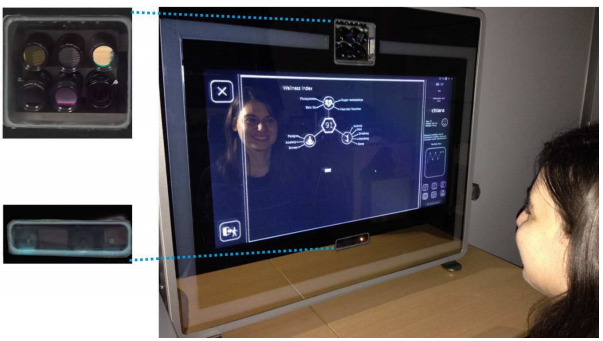
\includegraphics[width=12cm]{images/mirror.png}
    \caption{SEMEOTICONS\cite{andreu2015mirror}}
    \label{fig:seme}
\end{figure}
类似的,国外也有类似地考虑日常环境下面诊系统的系统设计。如图 \ref{fig:seme} 所示,Yasmina Andreu-Cabedo等 \cite{andreu2015mirror}开发了SEMEOTICONS系统。
SEMEOTICONS的系统设计与其他面诊系统区别点在于系统设计的出发点就是考虑到日常健康环境,而不是基于现有诊所环境下的面诊系统迁移到日常健康环境,同时对原型系统进行了用户调研。
SEMEOTICONS是一款放在家庭室内环境的镜子,通过摄像头和传感器采集面部信息和体温,监测与心血管疾病相关的疲劳、压力和焦虑等特征,让用户能够监测自己的健康情况,并根据量身定制的健康指南来改善用户的生活方式。
该系统由室内的硬件设备和远程服务器一起完成健康监测的功能,室内设备负责采集数据,远程服务器负责处理数据分析结果。
在生活中照镜子本来就是每个人的日常行为,该研究将面诊技术和健康管理结合起来,并且将应用场景拓展到了日常环境。
他们后续还进行了一次用户体验研究,研究结果表明\cite{coppini2017user} 他们的原型系统的设计被大多数用户所接受: 虽然测试过程非常耗时,大多数参与研究中的志愿者仍然很愿意完成并按计划进行实验,部分志愿者考虑了系统给出的健康指南,甚至因此改变了自己的生活方式。
总的来说,该系统通过将诊断和日常的照镜子的行为结合起来,可以很方便与用户的日常生活融合起来,同时在服务器端也可以方便的实现算法模型的适配和更新。
但是该系统固定在房间的某个位置使用的方式不够便携,同时该系统需要一系列的传感器设备,不仅增加了硬件的成本,部署起来也相对麻烦,而且只能在室内使用。

现有的面诊系统大多是为诊所环境设计,部分研究考虑到日常场景的使用问题,但没有系统地用人机交互的研究方法对日常场景下的用户使用进行研究,
将面诊技术应用到日常健康场景还需要进一步深入地探索。

\section{日常健康管理技术}

由上一节可知面诊技术的应用和研究有不少,但是它们很少关注日常健康场景。
而在人机交互领域,国内外有大量的关于如何设计日常健康场景下健康相关的交互研究。

从研究目的来看,日常健康技术的研究重心偏向于关注患者的日常生活体验,加强患者与医护人员的协作,提高用户的疾病认知等方面\cite{nunes2015self-care}。
从研究的出发点来看,主要可以分为慢性疾病管理和健康行为引导两种\cite{nunes2015self-care},本小节将从这两个方面展开分别介绍。

\subsection{慢性疾病管理}
随着医学、科技和社会的进步,当前的人们享受着比以往时代更加长寿的生活\cite{OlshanskyDEMOGRAPHY}。寿命的增加也间接地造成了慢性病患病率的提高\cite{world2012world}。慢性病作为一种长期的疾病,大多数在目前的医疗条件下是无法治愈的,但是可以通过适当的管理控制病情,因此慢性病管理变得格外重要。

在慢性疾病管理方面,当前研究主要是关于各种类型的慢性疾病的长期管理和追踪技术,用于支持慢性病患者及其护理人员了解病人的身体状态并加强对病情的控制,从而提高用户在患病状态下的生活品质。
如 Lena Mamykina\cite{burgermaster2019personal}团队在安卓平台上研发了一款称为 Platano 的应用,
该系统能够对用户的饮食纪录给出对应的反馈,并通过积分与金钱奖励等机制,逐渐改变用户的饮食习惯。经过实验发现该系统提供的功能能够大大鼓励用户完成血糖管理的任务(如严格控制饮食)。
Kiyoshi Yasuda等\cite{lazar2016evaluation}则研究了如何设计与痴呆病人的远程通讯系统,帮助痴呆病人与家人进行沟通,提高痴呆病人在家保持情绪稳定的时间,改善痴呆病人的日常在家的生活质量。
Amid Ayobi等\cite{ayobi2017quantifying} 通过对多发性硬化病人的日常监测应用的研究,发现日常健康技术可以帮助提高病人的日常控制意识,而不只是监测疾病相关的指标。

在精神健康方面,Jakob E. Bardram等\cite{bardram2013designing}探索了如何设计监测双相情感障碍症的日常应用,研究发现因为移动平台的便携性,患者可以随时携带智能手机,通过系统提醒和实时数据可视化可以提高患者的疾病意识。
同时该系统提供的评估功能相较于纸质表格评估的模式,使用体验大大得到了提高,更加利于用户长期坚持疾病评估。

总的来说,健康管理和患者的日常生活密切相关,慢性病患者需要调整自己的饮食和锻炼等来实现有效的健康管理\cite{nunes2018understanding},因此研究慢性病管理技术对提高慢性病患者的生活水平非常重要。
慢性病管理技术能够帮助用户了解病情的变化,及时对自己的病情变化做出应对行为,更好地评估自己的日常健康行为和更快地适应当前的生活状态\cite{ayobi2017quantifying}。


\subsection{健康行为引导}
在健康行为引导即鼓励用户健康生活方面,主要是对各类监测系统的研究。这类系统的功能主要是对用户的各种健康比较相关的指标,能够让用户得到关于自己健康情况的一个反馈,
让处于健康或者亚健康的情况下的用户更加健康地生活。这类监测相关的技术,从对用户监测的指标来看,可以大致分为两类:
\begin{enumerate}

    \item 日常行为的监控:通过监控用户的日常饮食、运动情况等日常行为,培养用户更好的饮食习惯、锻炼习惯等\cite{purpura2011fit4life, Inagawa2013A,bravata2007using,cordeiro2015barriers,lin2006fish, miller2014stepstream}。 例如Yuma Inagawa等人\cite{Inagawa2013A} 开发了一个营养管理和检索系统,根据用户的喜好给出推荐的菜单,用户也可以给出对应的反馈,以此来培养用户健康的健康饮食的观念,进而达到引导用户的行为的效果。

    \item 健康指标的监控:健康指标主要包括生命体征如呼吸、血压、心率,也包括睡眠、体重等\cite{kay2012lullaby, gronvall2013beyond}。
    
\end{enumerate}

例如Stephen Purpura等人\cite{purpura2011fit4life} 利用内有传感器的眼镜、耳机,臂环等可穿戴设备,通过记录用户的饮食、心率、咀嚼动作、体重、血压等健康指标,设计了一个鼓励用户减肥的系统 fit4life; 
Lullaby\cite{kay2012lullaby}是Matthew Kay等人利用光线、声音、温度、运动等传感器研发出来,用于研究干扰用户睡眠因素的系统。
Lullaby系统通过记录和可视化用户的睡眠状态,能够帮助用户识别睡眠中断和环境因素之间的联系。 

% 总结上述的研究本文发现,当前关于日常健康交互技术的研究有很多,涉及各种慢性疾病管理以及各种健康评估和监测的方法,但是目前还缺乏关于日常环境下如何设计基于面部信息进行健康评估的研究。

目前这些日常场景下的健康追踪和监测技术,主要的实现方式还是通过量化采集用户的健康指标相关的数据。
那么如何利用其他的健康相关数据,如面部信息,来支持用户的日常健康,在人机交互领域还没有得到深入研究。
总的来说,面诊技术在日常健康场景下的应用还是一个新的研究问题,但人机交互中的关于日常健康场景成熟的研究方法本文值得借鉴。


\section{本章小结}
本章前半部分主要介绍了当前主要的面诊系统设计已经各自的特点和不足,尤其在日常健康场景的系统设计研究目前还十分欠缺。
人机交互领域在日常健康方面的很多研究值得借鉴,因此本章后半部分介绍了人机交互领域从传统的慢性疾病管理到健康行为引导的研究,
同时指出当前的日常健康的研究还未探索面部信息作为健康指标的不足不处。
本文将在下一章节使用人机交互的研究方法,对日常健康场景下系统如何设计的问题进行探索。